
\chapter{Python 的操作基础}

\section{Python 的常用数据类型}

Python 的常用数据类型有:数字,字符串,列表,元组,字典。

\subsection{数字类型:整数型,浮点型}

Python 中定义一个数字型变量特别方便,直接用等号赋值。例如:

\begin{lstlisting}[Language=Python]
In [16]: a = 1

In [17]: a
Out[17]: 1

In [18]: b = 2.2

In [19]: b
Out[19]: 2.2
\end{lstlisting}

在上面的这段代码中,定义了一个数字型变量 a,并将其赋值为 1;定义了一个浮点型变量 b,并将其赋值为 2.2。


Python 并不像其他的一些编程语言那样需要明确数字的细分类型:整数型(int),浮点型(float)等。Python 可以自己判断数字类型,例如在上面的代码中,由于 a 没有小数点,Python 认为 a 是整数型,b 带了小数点,Python 认为 b 是浮点型,我们可以利用 type 函数检验下:

\begin{lstlisting}[Language=Python]
In [20]: type(a)
Out[20]: int

In [21]: type(b)
Out[21]: float
\end{lstlisting}


Python 中数字类型的互换也非常方便,只需要将数据类型作为函数名即可,如下面代码:

\begin{lstlisting}[Language=Python]
In [3]: float(a) # 将整形数据 a 转化为浮点型数据
Out[3]: 1.0

In [4]: int(b) # 将浮点型数据 b 转化为整形数据
Out[4]: 2
\end{lstlisting}

对于四则运算:加减乘除,则用 + - * / 符号直接输入即可:

\begin{lstlisting}[Language=Python]
In [22]: 1 + 2
Out[22]: 3

In [23]: 20 - 5 * 2
Out[23]: 10

In [24]: (10 - 5) / 2
Out[24]: 2.5

In [25]: 9 / 5
Out[25]: 1.8
\end{lstlisting}

求余数用百分号~ \%,幂运算用两个星号 **,例如:

\begin{lstlisting}[Language=Python]
In [26]: 8 % 5
Out[26]: 3

In [27]: 3 ** 2
Out[27]: 9
\end{lstlisting}

对数字类型还有一些其他运算,例如求绝对值用函数 abs(),四舍五入函数用 round(),求最大值函数 max(),求最小值函数 min():

\begin{lstlisting}[Language=Python]
In [28]: abs(-2.5)
Out[28]: 2.5

In [29]: round(3.4)
Out[29]: 3

In [30]: round(3.45, 1) # 四舍五入保留一位小数
Out[30]: 3.5

In [31]: max(10, 20)
Out[31]: 20

In [32]: min(10, 20)
Out[32]: 10
\end{lstlisting}

更复杂的数学运算需要调用数学包 math,基本能满足所有的数学运算,例如:

\begin{lstlisting}[Language=Python]
In [6]: import math

In [7]: math.sin(math.pi/2) # 正弦函数
Out[7]: 1.0

In [8]: math.log10(100) # 对数函数
Out[8]: 2.0
\end{lstlisting}

第一行代码调用 math 中的 sin 函数求 $sin(\pi/2)$,其中调用了 math 中的 pi 函数表示 $\pi$,第二行代码调用了对数函数求 $\ln(100)$。

\subsection{字符串类型}

字符串也是 Python 中比较常见的数据类型,可以用单引号或双引号表示字符串。例如:

\begin{lstlisting}[Language=Python]
In [33]: name = "chen"

In [34]: name
Out[34]: 'chen'

In [35]: city = 'Beijing'

In [36]: city
Out[36]: 'Beijing'
\end{lstlisting}

字符串的拼接直接用加号 + 即可:

\begin{lstlisting}[Language=Python]
In [3]: name+city
Out[3]: 'chenBeijing'
\end{lstlisting}

还有一种常用的拼接方式是用 join 方法:str.join(sequence),将序列中的元素以指定的字符连接生成一个新的字符串。例如:

\begin{lstlisting}[Language=Python]
In [28]:  ','.join(['chen', 'zhang', 'li'])  # 将三个字符串用逗号拼接
Out[28]: 'chen,zhang,li'

In [29]: '-'.join(['2020', '05', '13'])  # 将三个字符串用横线拼接
Out[29]: '2020-05-13
\end{lstlisting}

若重复输出字符串,可以使用星号 *:

\begin{lstlisting}[Language=Python]
>>> name = 'chen'
>>> name * 2
'chenchen'
\end{lstlisting}

可以将字符串视为一个数组,利用数组的索引得到字符串中的字符,例如:

\begin{lstlisting}[language=python]
In [37]: name[0] # 0 代表第 1 个索引
Out[37]: 'c'

In [38]: name[0:3] # 截取字符串中的一部分,遵循“左闭右开”原则,得到第 1 到第 3 个字符
Out[38]: 'che'
\end{lstlisting}

判断某个字符或某段字符串是否在字符串中,可以用 in 或 not in:

\begin{lstlisting}[Language=Python]
In [39]: 'c' not in name
Out[39]: False

In [40]: 'Bei' in city
Out[40]: True
\end{lstlisting}

Python 中字符串的常用运算符由下表展示:

\begin{center}
\begin{tcolorbox} [title = 字符串的常用运算符]
  \centering
  \begin{tcboutputlisting}
  \begin{tabular}{>{\bfseries}ll}
    + &字符串拼接\\
    *&重复输出字符串\\
    $[]$ &通过索引获取字符串中字符,str[1] 是第 2 个字符\\
    $[ : ]$ & 截取一部分字符串,遵循“左闭右开”原则,str[0,2] 不包含第 3 个字符\\
  in &如果字符串中包含给定的字符返回 True\\
  not in &如果字符串中不包含给定的字符返回 True
  \end{tabular}
\end{tcboutputlisting}
\end{tcolorbox}
\end{center}

Python 中常用的字符串处理函数有:

\begin{center}
\begin{tcolorbox} [title = 字符串的常用处理函数]
  \centering
  \begin{tcboutputlisting}
  \begin{tabular}{>{\bfseries}ll}
    capitalize(str) &将字符串 str 内容转为大写\\
    lower(str)&将字符串 str 内容转为小写\\
    len(str) &字符串 str 的长度\\
    isnumeric(str) & 如果字符串 str 中只包含数字字符,则返回 True,否则返回 False\\
  isalpha(str) &如果字符串 str 的字符都是字母则返回 True, 否则返回 False
  \end{tabular}
\end{tcboutputlisting}
\end{tcolorbox}
\end{center}

\subsection{列表类型}

列表(List)是最常用的 Python 数据类型,它由一个\textbf{中括号} [ ] 以及逗号分隔的不同数值或字符串组成,例如:

\begin{lstlisting}[Language=Python]
In [1]: list1 = [34, 10, 25]

In [2]: list1
Out[2]: [34, 10, 25]

In [3]: list2 = ['chen', 'zhang', 'wang']

In [4]: list2
Out[4]: ['chen', 'zhang', 'wang']

In [5]: list3 = [10, 'wang', 33]

In [6]: list3
Out[6]: [10, 'wang', 33]
\end{lstlisting}

与字符串的索引一样,列表索引从 0 开始,第一个值的索引是位置 0,第二个索引是 1,依此类推。

\begin{lstlisting}[Language=Python]
In [7]: list1[0] # list1 的第 1 个元素
Out[7]: 34

In [8]: list2[1] # list2 的第 2 个元素
Out[8]: 'zhang'

In [9]: list1[0:2] # “左闭右开”原则,list1 第 1 到第 2 个元素
Out[9]: [34, 10]

In [10]: list1[0:] # list1 第 1 到之后的所有元素
Out[10]: [34, 10, 25]
\end{lstlisting}

另外,\textbf{Python 支持倒序索引},-1 表示倒数第 1 个元素,-2 表示倒数第 2 个元素,依次类推。

\begin{lstlisting}[Language=Python]
>>> list1[-1] # list1 的倒数第 1 个元素
25
>>> list2[-2] # list2 的倒数第 2 个元素
'zhang'
\end{lstlisting}

更改列表某个位置的元素,可以直接用索引更改。

\begin{lstlisting}[Language=Python]
In [9]: list = [21, 16, 30]

In [10]: list[1] = 10 # 将 list 第 2 个元素更改为 10

In [11]: list
Out[11]: [21, 10, 30]
\end{lstlisting}

删除列表某个索引的元素,用 del:

\begin{lstlisting}[Language=Python]
>>> list = [34, 46, 23]
>>> del list[1]
>>> list
[34, 23]
\end{lstlisting}

对于列表类型,运算符 + 、*、in、not in 的功能与字符串中的功能相同。下面举例说明:

\begin{lstlisting}[Language=Python]
>>> list = [13, 23]
>>> list = list + [21, 65]
>>> list
[13, 23, 21, 65]
>>> list * 2
[13, 23, 21, 65, 13, 23, 21, 65]
>>> 12 in list
False
>>> 12 not in list
True
\end{lstlisting}

列表类型还有很多函数可以使用:

\begin{lstlisting}[Language=Python]
In [12]: list = [34, 46, 23]

In [13]: list.append(3) # 在列表末尾添加一个元素

In [14]: list
Out[14]: [34, 46, 23, 3]
[34, 46, 23, 3]

>>> list.insert(1, 10) # 在列表第二个位置添加一个元素 10
>>> list
[34, 10, 46, 23, 3]

>>> list.extend([4, 5, 6]) # 将另一个列表(元组类型也可以)添加到该列表末尾
>>> list
[34, 10, 46, 23, 3, 4, 5, 6]
\end{lstlisting}

列表类型的其他函数还有:
\begin{center}
\begin{tcolorbox} [title = 列表类型的一些处理函数]
  \bf
  \begin{tcboutputlisting}
  \begin{tabular}{>{\bfseries}ll}
    max(list) &返回列表 list 中的最大值元素\\
    min(list)&返回列表 list 中的最小值元素\\
    list.append(obj) &在列表末尾添加新的对象\\
    list.extend(seq) & 在列表末尾一次性追加另一个序列中的多个值\\
    list.insert(index, obj) & 将对象插入列表\\
    list(seq) & 将元组转化为列表\\
    len(list) &返回列表 list 的长度\\
    list.count(obj) & 统计某个元素在列表中出现的次数\\
  list.reverse() &将列表反转\\
  list.clear() & 清空列表
  \end{tabular}
\end{tcboutputlisting}
\end{tcolorbox}
\end{center}

\subsection{元组类型}

Python 的元组(tuple)与列表类似,不同之处在于\textbf{元组的元素不能修改}。元组使用\textbf{小括号}创建,并使用逗号隔开。访问列表元素或者截取部分元组与列表非常类似:

\begin{lstlisting}[Language=Python]
In [15]: tup = (13, 'zh', 20)

In [16]: tup[1]
Out[16]: 'zh'

In [17]: tup[0:2]
Out[17]: (13, 'zh')

In [18]: tup[0:]
Out[18]: (13, 'zh', 20)
\end{lstlisting}

元组中的元素不能修改,但可以用 del 删除整个元组, 也可以用运算符 +、*、in、not in:

\begin{lstlisting}[Language=Python]
>>> tup = (13, 'zh', 20)
>>> del tup # tup 已经被完全删除了,需要重新创建
>>> tup = (23, 45, 21)
>>> tup = tup + (32, 21)
>>> tup
(23, 45, 21, 32, 21)
>>> tup * 2
(23, 45, 21, 32, 21, 23, 45, 21, 32, 21)
>>> 25 in tup
False
>>> 25 not in tup
True
\end{lstlisting}

元组类型的其他函数还有:
\begin{center}
\begin{tcolorbox} [title = 元组类型的一些处理函数]
  \bf
  \begin{tcboutputlisting}
  \begin{tabular}{>{\bfseries}ll}
    max(tup) &返回元组 tup 中的最大值元素\\
    min(tup)&返回元组 tup 中的最小值元素\\
    tuple(seq) & 将列表转化为元组\\
    len(tup) &返回元组 tup 的长度,即元素个数\\
    tup.count(obj) & 统计某个元素在元组 tup 中出现的次数\\
  \end{tabular}
\end{tcboutputlisting}
\end{tcolorbox}
\end{center}


\subsection{字典类型}

字典是另一种可变容器模型,字典的每个“键值 (key : value) 对”用冒号 : 分割,每个对之间用逗号分割,整个字典包括在\textbf{花括号} { } 中。\textbf{键(key)必须是唯一且不可变},但值(value)可以取任何数据类型,也可以改变。

\begin{lstlisting}[Language=Python]
In [19]: dict = {'name' : 'chen', 'mark' : 95}

In [20]: dict
Out[20]: {'name': 'chen', 'mark': 95}
\end{lstlisting}

访问字典里的值时,则把相应的键放入到方括号中:

\begin{lstlisting}[Language=Python]
In [21]: dict['name']
Out[21]: 'chen'

In [22]: dict['mark']
Out[22]: 95
\end{lstlisting}

修改字典里的值时,则把相应的键放入到方括号中,赋值进行修改即可:

\begin{lstlisting}[Language=Python]
In [23]: dict['name'] = 'wang'

In [24]: dict['mark'] = 80

In [25]: dict
Out[25]: {'name': 'wang', 'mark': 80}
\end{lstlisting}

删除字典里的某个键值时,用 del:

\begin{lstlisting}[Language=Python]
>>> del dict['name']
>>> dict
{'mark': 80}
\end{lstlisting}

注意:键必须不可变,所以可以用数字,字符串或元组充当,但用列表就不行。

\begin{lstlisting}[Language=Python]
>>> dict1 = {'name': 'zhang', 123 : 45, (1, 2): 10}
>>> dict1
{'name': 'zhang', 123: 45, (1, 2): 10}
>>> dict2 = {[1, 2, 3] : 10} # 用列表做键出现错误
Traceback (most recent call last):
  File "<input>", line 1, in <module>
TypeError: unhashable type: 'list'
\end{lstlisting}


字典类型的常用函数还有:
\begin{center}
\begin{tcolorbox} [title = 字典类型的一些处理函数]
  \bf
  \begin{tcboutputlisting}
  \begin{tabular}{>{\bfseries}ll}
    len(dict) &返回字典 dict 中的元素个数,即键或值的个数\\
    dict.clear() &删除字典 dict 中的所有元素\\
    key in dict & 如果键 key 在字典 dict 里返回 true,否则返回 false\\
    dict.values() & 返回一个迭代器,可以使用 list() 来转换为列表\\
  dict.keys()  & 返回一个迭代器,可以使用 list() 来转换为列表
  \end{tabular}
\end{tcboutputlisting}
\end{tcolorbox}
\end{center}


\subsection{集合类型}

集合(set)是一个无序的\textbf{不重复}元素序列,一般使用大括号 { } 创建(注意:创建一个空集合必须用 set() 而不是 { },因为 { } 默认创建一个空字典)。

\begin{lstlisting}[Language=Python]
In [28]: set1 = {34, 23, 'chen'}

In [29]: set1
Out[29]: {23, 34, 'chen'}

In [30]: set2 = {12, '34', 10}

In [31]: set2
Out[31]: {10, 12, '34'}
\end{lstlisting}

集合间的常用运算符包括:

\begin{center}
\begin{tcolorbox} [title = 集合间的常用运算符]
  \bf
  \begin{tcboutputlisting}
  \begin{tabular}{>{\bfseries}ll}
    - &减号左边集合包含,而减号右边不包含的元素\\
    | &两个集合的并集\\
    \& & 两个集合的交集\\
    $\land$ & 不同时包含于两个集合中的元素\\
  \end{tabular}
\end{tcboutputlisting}
\end{tcolorbox}
\end{center}

\begin{lstlisting}[Language=Python]
>>> set1 = {34, 12, 'chen'}
>>> set2 = {12, 'wang', 10}
>>> set1 - set2
{34, 'chen'}
>>> set1 | set2
{34, 'wang', 10, 'chen', 12}
>>> set1 & set2
{12}
>>> set1 ^ set2
{'wang', 34, 10, 'chen'}
\end{lstlisting}

在集合中添加元素可以用 add 函数,添加多个元素(可以是列表、元组或字典)用 update 函数,删除某个元素用 remove 函数, 判断某个元素是否在集合中,用 in 或 not in:

\begin{lstlisting}[Language=Python]
>>> set = {13, 45, 67}
>>> set.add(10)
>>> set
{10, 67, 45, 13}
>>> set.remove(10)
>>> set
{67, 45, 13}
>>> set.update([80, 44])
>>> set
{67, 44, 45, 13, 80}
>>> 44 in set
True
>>> 44 not in set
False
\end{lstlisting}

集合类型的常用函数还有:
\begin{center}
\begin{tcolorbox} [title = 集合类型的一些处理函数]
  \bf
  \begin{tcboutputlisting}
  \begin{tabular}{>{\bfseries}ll}
    len(set) &返回集合 set 中的元素个数\\
    set.add() &向集合 set 中添加一个元素\\
    set.remove() & 集合中移除一个元素\\
    set.update(seq) & 添加多个元素,可以是列表、元组或字典\\
  set1.issubset(set2)  & 判断集合 set1 是否为另一个集合 set2 的子集\\
  set1.issuperset(set2)  & 判断集合 set1 是否为另一个集合 set2 的父集\\
  set1.isdisjoint(set2) & 判断两个集合是否包含相同的元素,如果没有返回 True\\
  set1.union(set2) & 返回两个集合的并集
  \end{tabular}
\end{tcboutputlisting}
\end{tcolorbox}
\end{center}

\subsection{布尔值,数据类型转换}

Python 中的布尔值(Bool) 一般通过逻辑判断产生,只有两个可能的结果:True 或 False。

\begin{lstlisting}[Language=Python]
In [5]: 10 > 3
Out[5]: True

In [6]: 3 == 4
Out[6]: False
\end{lstlisting}

在做逻辑判断时,两个等号 == 表示是否相等,若仅有一个等号,则表示赋值。另外,python 中提供了 is 关键字,作用与 == 相同。

\begin{lstlisting}[Language=Python]
In [19]: a = 3  # 一个等号表示将 a 赋值为 3

In [20]: a == 4  # 两个等号表示判断 a 是否等于 4
Out[20]: False

In [21]: a is 3  # is 与 == 相同,判断是否相等
Out[21]: True

In [22]: a is 4
Out[22]: False
\end{lstlisting}

对多个逻辑判断的运算,即 ``且”,``或”,``非”, python 分别提供了 and, or, not:

\begin{lstlisting}[Language=Python]
In [7]: 10 > 3 and 3 > 2
Out[7]: True

In [8]: 10 > 3 and 3 > 4
Out[8]: False

In [9]: 10 > 3 or 3 > 4
Out[9]: True

In [10]: not 3 > 4
Out[10]: True
\end{lstlisting}

有时候经常需要对一些数据进行类型转换,python 提供了一些转换函数。

\begin{center}
\begin{tcolorbox} [title = python 的一些类型转换函数]
  \bf
  \begin{tcboutputlisting}
  \begin{tabular}{>{\bfseries}ll}
    int() &将一个数据转化为整数型\\
    float() & 将一个数据转化为浮点型\\
        str() &将一个数据转化为字符串\\
  \end{tabular}
\end{tcboutputlisting}
\end{tcolorbox}
\end{center}

举例:

\begin{lstlisting}[Language=Python]
In [26]: int(3.5)
Out[26]: 3

In [27]: float(3)
Out[27]: 3.0

In [30]: str(3.5)  # 将数字转化为字符串
Out[30]: '3.5'
\end{lstlisting}

\section{Python 输出输入}
\subsection{print, input 函数}

Python 输出非常方便,用 print() 函数,小括号里面可以是数字、字符串、列表、字典等类型。

\begin{lstlisting}[Language=Python]
In [34]: print([12, 45, 69])
[12, 45, 69]

In [35]: print({'name' : 'chen', 'mark' : 85})
{'name': 'chen', 'mark': 85}

In [41]: a = {4, 5, 6}

In [42]: print(a)
{4, 5, 6}
\end{lstlisting}

若要格式化输出,要用到百分号 \%,语法规则类似 c 语言。

\begin{lstlisting}[Language=Python]
In [36]: import math

In [37]: print('the number is %d' % math.pi) # 按照整数输出
the number is 3

In [38]: print('the number is %.2f' % math.pi) # 按照浮点数输出,并保留 2 位小数
the number is 3.14

In [39]: print('the number is %.2f\n' % math.pi) # \n 表示输出后光标换行
the number is 3.14

In [13]: print('the number is %5.2f' % math.pi)# 按照浮点数输出,保留 2 位小数,并且输出内容的宽度为5个字符
the number is  3.14

In [40]: print('the number is %s' % 321) # 按照字符串输出
the number is 321


\end{lstlisting}

引号里面的百分号~\% 定义了输出数据的格式,\%d 表示按整数类型输出, \%.2f 表示按浮点型输出,其中小数点后的数字表示保留几位小数,小数点前的数字表示输出变量所占的字符宽度,\%s 表示按字符串输出。

自从版本 3.6 之后, python 新增了 print(f`\{expression\}') 的用法,大括号中的 exression 可以是一个变量名,例如,下面的代码打印出一个数组列表:


\begin{lstlisting}[Language=Python]
In [1]: a = [1, 2, 3]

In [2]: print(f'the array is {a}') # 输出列表 a
the array is [1, 2, 3]
\end{lstlisting}

exression 也可以是变量名后面跟上冒号格式化输出,类似百分号\% 的格式化出输出。

\begin{lstlisting}[Language=Python]
In [10]: a = 3.1415926

In [11]: print(f'the array is {a:5.2f}') # 将变量 a 保留两位小数,5个字符的宽度输出
the array is  3.14
\end{lstlisting}



Python 中的输入用 input 函数,可以用户从键盘输入中读取文本,例如:

\begin{lstlisting}[Language=Python]
In [44]: str = input('input your name:')

input your name:chen

In [45]: str
Out[45]: 'chen'
\end{lstlisting}

\subsection{读写文件}

Python 用 open() 函数返回一个文件对象,常用的语法规则为:

\begin{center}
\begin{tcolorbox}[title = open 函数的语法]
\textbf{open(filename, mode)}
\tcblower
\vspace{10pt}
\begin{tcboutputlisting}
\begin{tabular}{>{\bfseries}ll}
  filename &字符串,文件地址及文件名,默认地址为当前的项目文件夹\\
  mode & 文件读写模式,默认模式为只读(r)
\end{tabular}
\end{tcboutputlisting}
\tcbuselistingtext

\end{tcolorbox}
\end{center}

常见的文件读写模式(mode)有:

\begin{center}
\begin{tcolorbox}[title = 常用的文件读写模式(mode)]
\textbf{open(filename, mode)}
\tcblower
\vspace{10pt}
\begin{tcboutputlisting}
\begin{tabular}{>{\bfseries}ll}
  r & 以只读方式打开文件,从文件内容开头读取,这是默认模式\\
  \specialrule{0em}{1pt}{1pt}
  \multirow{2}*{w} &打开一个文件只用于写入,从文件内容开头写入,即原有内容会被删除;\\
  &如果该文件不存在,创建新文件\\
  \specialrule{0em}{1pt}{1pt}
  \multirow{2}*{w+} &打开一个文件用于读写,从文件内容开头写入,即原有内容会被删除;\\
  &如果该文件不存在,创建新文件\\
  \specialrule{0em}{1pt}{1pt}
r+	&打开一个文件用于读写。文件指针将会放在文件的开头\\
\multirow{2}*{a}	 &打开一个文件用于追加写入,如果该文件已存在,从文件结尾写入;\\
 &如果该文件不存在,创建新文件进行写入\\
   \specialrule{0em}{1pt}{1pt}
 \multirow{2}*{a+}	 &打开一个文件用于追加读写,如果该文件已存在,从文件结尾写;\\
 &如果该文件不存在,创建新文件进行写入
\end{tabular}
\end{tcboutputlisting}
\tcbuselistingtext

\end{tcolorbox}
\end{center}

上面几个读写模式的详细比较如下面的表格所示:


\begin{table}[!ht]
  \centering
  \caption{读写模式比较}
  \begin{tabular}{|c|c|c|c|c|c|c|}
    \hline
    模式 & r &r+ & w & w+ &a & a+\\
    \hline
    读&\checkmark &\checkmark &&\checkmark&&\checkmark\\\hline
    写& &\checkmark&\checkmark&\checkmark&\checkmark&\checkmark \\\hline
    创建& & &\checkmark&\checkmark&\checkmark&\checkmark\\\hline
    覆盖&&&\checkmark&\checkmark&&\\\hline
    从文件开始操作&\checkmark&\checkmark&\checkmark&\checkmark&&\\\hline
    在文件末尾操作& & & & &\checkmark&\checkmark \\\hline
  \end{tabular}
\end{table}

举例:

\begin{lstlisting}[Language=Python]
f = open('F:/text.txt', 'w') # 在指定位置(F盘)新建文件
f.write('my name is zhang san\n his name is li si') # 书写内容,用 \n 换行
f.close() # 关闭打开的文件
\end{lstlisting}

上面的程序在 F 盘新建了一个 txt 文件,也可以直接写文件名字,这样文件就默认建立在当前 Python 项目的文件夹下。 通过 write() 函数在文件里面写内容,其中,$\backslash$\text{n} 表示内容换行。通过 read() 函数读取文件里的全部内容,并返回一个字符串:

\begin{lstlisting}[Language=Python]
f = open('F:/text.txt', 'r') # 在指定位置新建文件
str = f.read() # 读取文件内容
print(str) # 将内容输出到屏幕
f.close() # 关闭打开的文件
\end{lstlisting}

如果只读取一行,可以用 readline() 函数,另外可以用 readlines() 函数读取所有行,并返回一个字符串列表。

在实际的 python 读写文件中,经常用到的是 with-open 语句。由于文件读写时都有可能产生 IOError,一旦出错,后面的 f.close() 就不会调用,用 with-open 语句可以省略 f.close() 语句。上面的读写代码也可以变为:

\begin{lstlisting}[Language=Python]
# 读文件
with open ('F:/text.txt', 'r') as f:
     str = f.read() # 读取文件内容
     print(str) # 将内容输出到屏幕

# 写文件
with open('F:/text.txt', 'w') as f:
     f.write('my name is zhang san\n his name is li si')
\end{lstlisting}




\section{Python 编写程序}

Python 编写程序时,一般有多行代码,因此一般在 Python 编辑器里面的 Editor 中写。下面我们以 Spyder 为例,展示如何使用里面的 Editor 书写程序(Pycharm 中如何使用 Editor 新建书写程序文件可以翻看本书第一章)。

在 Spyder 左上角的文件夹栏中,选择一个文件夹(或者自己新建一个文件夹)(该文件夹即为我们 python 程序文件存放的位置),然后单击右键,新建一个 module 文件,即为 python 的程序文件,然后在弹出的窗口中,输入 python 程序文件的名字,如下图所示:


\begin{figure}[!ht]
  \centering
  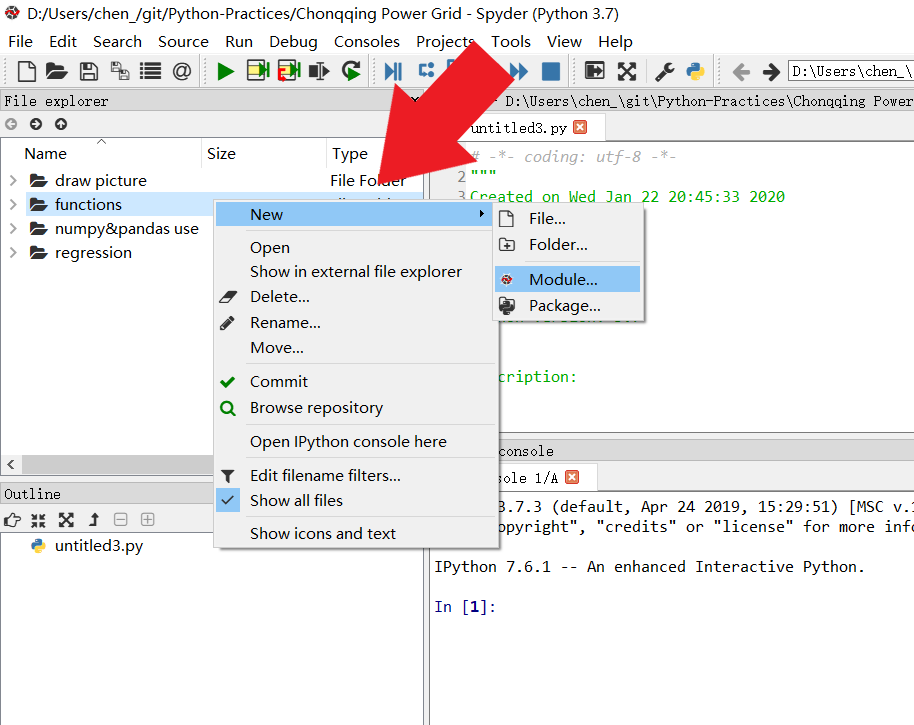
\includegraphics[width=6cm, height=6cm]{figure/function1.png}~~~~
  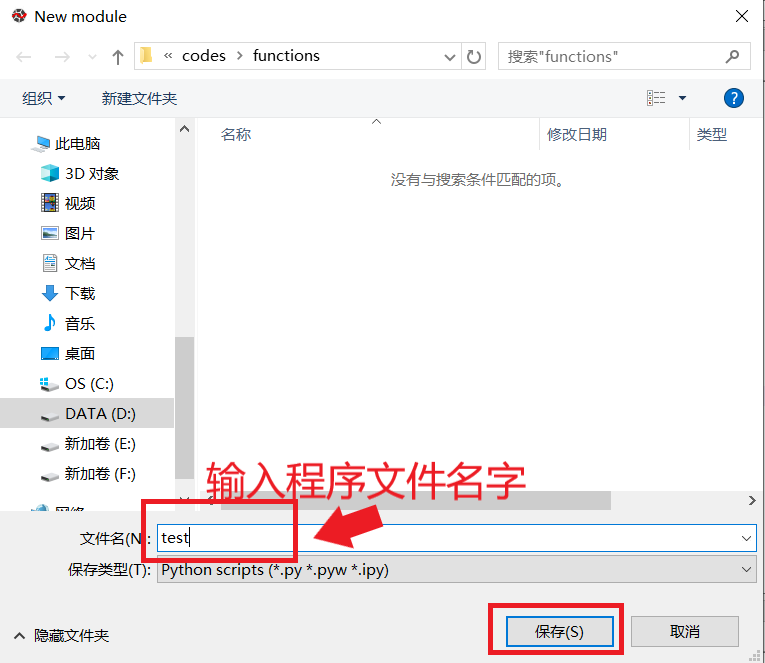
\includegraphics[width=6cm, height=6cm]{figure/function2.png}
\end{figure}


Python 中程序文件的格式为 py,假设我们命名程序文件为 test,则 Editor 窗口中会自动打开 test.py 文件,就可以在里面输入代码了。


\begin{figure}[!ht]
  \centering
  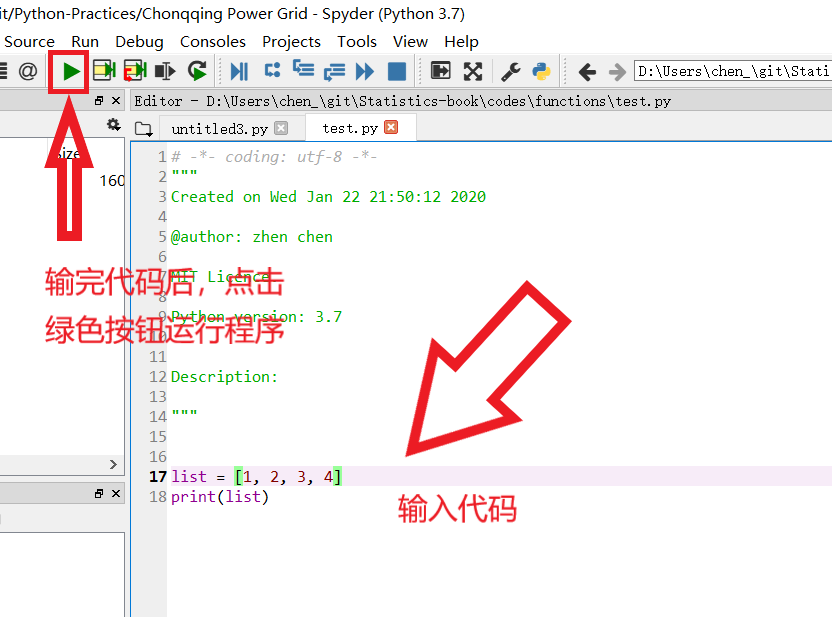
\includegraphics[scale = 0.3]{figure/function3.png}
\end{figure}

假设在 test.py 文件中输入一下代码,

\begin{lstlisting}[Language=Python]
list = [1, 2, 3, 4]
print(list)
\end{lstlisting}

运行程序后,就能在 Spyder 的控制台(Console)窗口看到输出的结果,在上面的程序中,我们输出打印了一个列表。

\subsection{语句缩进}

Python 与许多其他编程语言的区别在于:Python 使用缩进或对齐表示不同的代码块,而不是用分号或大括号。例如:

\begin{figure}[!ht]
  \centering
  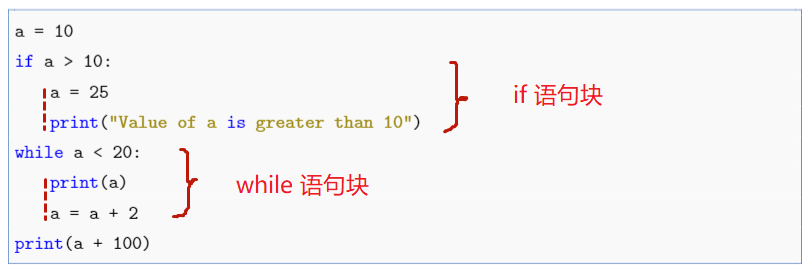
\includegraphics[scale = 0.9]{figure/codeStyle.png}
\end{figure}

该命令的输出结果为:

\begin{lstlisting}[Language=Python]
10
12
14
16
18
120
\end{lstlisting}

在上面的语句中,if 语句块(代码块)有相同的缩进,while 语句块也有相同的缩进,不同的语句块增加了程序的可读性,并且让我们知道不同命令语句的作用范围。例如,语句 print("Value of a is greater than 10") 与 a = 25 对齐,他们都属于 if 语句块,所以它们只在 if 语句块里面运行,假如 print("Value of a is greater than 10") 不与 a = 25 对齐,而是与语句 a = 10 对齐:

\begin{lstlisting}[Language=Python]
a = 10
if a > 10:
    a = 25
print("Value of a is greater than 10")
while a < 20:
    print(a)
    a = a + 2
print(a + 100)
\end{lstlisting}

则该 print 语句不在 if 语句块中运行,而是在其外面运行,它的运行结果为:

\begin{lstlisting}[Language=Python]
Value of a is greater than 10
10
12
14
16
18
120
\end{lstlisting}

可以看出,把语句 print("Value of a is greater than 10") 放到外面时,该语句被执行了,而放在 if 语句块时,由于不满足 if 语句的判断条件,该语句没有被执行。

\subsection{条件语句}

编写程序时,经常用到一些条件或判断,需要用到 if 语句,它的字面意思是:如果(if)满足条件,做什么,否则(else)做什么。

例如,下面一段代码:

\begin{lstlisting}[Language=Python]
a = 10
if a > 10:
    print("Value of a is greater than 10")
else:
    print("Value of a is not greater than 10")
\end{lstlisting}

这段代码的意思是,如果 a 比 10 大,则输出 "Value of a is greater than 10",否则输出 "Value of a is not greater than 10"。if 语句还可以跟 elif (else if 的意思),再次判断一个条件。

\begin{center}
\begin{tcolorbox} [title = if 语句的一般模式]
  \bf
  \begin{tcboutputlisting}
    if 条件1:

        \quad statement\_block\_1

    elif 条件2:

        \quad statement\_block\_2

    else:

        \quad statement\_block\_3
\end{tcboutputlisting}
\end{tcolorbox}
\end{center}


上面 if 语句块的执行顺序为:如果条件1 为真,将执行 "statement\_block\_1" 块语句,如果条件1 为假,将判断 "条件2",如果条件2 为真,将执行 "statement\_block\_2" 块语句,如果条件2 为假,将执行"statement\_block\_3"块语句。举例:

\begin{lstlisting}[Language=Python]
wage = int(input("请输入你的月薪: "))
print("")
if wage <= 3000:
    print("贫困户")
elif wage <= 12000:
    print("平均水平")
else:
    print("土豪")
\end{lstlisting}

上面语句的意思是,若输入的月薪小于 3000,则输出“贫困户”,否则若月薪在 3000 与 12000 之间,输出“平均水平”,若月薪在 12000 之上,则输出“土豪”。

if 语句里面还可以嵌套 if 语句,进一步增加判断条件,举例:

\begin{lstlisting}[Language=Python]
wage = int(input("请输入你的月薪: "))
print("")
if wage <= 3000:
    print("贫困户")
    if 2000 <= wage < 3000:
        print("贫困户中的一般贫")
    if wage <= 1000:
        print("贫困户中的特贫")
else:
    print("不是贫困户")
\end{lstlisting}

在上面的程序中,若月薪小于等于 3000,又嵌套了两个条件进一步判断。

if 中条件判断中常用的符号有:>(大于), <(小于), >=(大于等于), <=(小于等于), ==(等于), !=(不等于)。需要注意的是,在编程语言的判断语句中,两个等号 == 表示判断是否相等(a == 3 表示判断 a 是否等于 3),而一个等号 = 表示的是变量赋值(a = 3 表示将 a 赋值为 3)。

\subsection{循环语句}

循环语句一般有两种,for 语句与 while 语句。for 循环可以遍历任何序列的项目,如一个列表、元组、集合或者一个字符串。for循环的一般格式如下:

\begin{center}
\begin{tcolorbox} [title = for 循环的一般格式]
  \bf
  \begin{tcboutputlisting}
    for <variable> in <sequence>:

    \quad~ <statements>
\end{tcboutputlisting}
\end{tcolorbox}
\end{center}

for 循环的作用是:遍历序列(sequence)中的所有元素,执行命令语句 statements,举例:

\begin{lstlisting}[Language=Python]
for i in range(3):
    print(i)
\end{lstlisting}

输出结果为 0, 1, 2,上述代码的作用是,对于 range(3) 中的每一个元素,打印元素。\textbf{for 循环经常结合序列函数 range() 一起使用}:range(a) 表示从 0 到 a-1 的一个数列,range(a, b) 表示从 a 到 b-1 的一个数列,range(a, b, c) 表示从 a 到 b-1,步长为 c 的一个数列。

另一个 while 循环语句的一般格式为:
\begin{center}
\begin{tcolorbox} [title = while 循环的一般格式]
  \bf
  \begin{tcboutputlisting}
    while 判断条件:

    \quad~ <statements>
\end{tcboutputlisting}
\end{tcolorbox}
\end{center}

它的作用是,只要满足 while 的判断条件,则一直执行 while 下面的执行语句 <statements>,举例:

\begin{lstlisting}[Language=Python]
a = 1
while a < 4:
    print(a)
    a = a + 1
\end{lstlisting}

输出结果为:1,2,3,上面语句的作用是:只要 a 小于 4,则将 a 值打印出来并将 a 值加 1,在 a 等于 4 时停止执行 while语句。

for 循环与 while 循环经常结合 break 或 continue 语句,break 语句可以跳出循环体,而continue 语句用来告诉 Python 跳过当前循环块中的剩余语句,然后继续进行下一轮循环。举例:

\begin{lstlisting}[Language=Python]
for i in range(3):
   if i == 1:
       break
   print(i)
print('循环结束')
\end{lstlisting}

输出结果如下,上面代码中 在 i 等于 1 时执行 break 跳出了整个循环体。

\begin{lstlisting}[Language=Python]
0
循环结束
\end{lstlisting}

若改为 continue 语句:
\begin{lstlisting}[Language=Python]
for i in range(3):
   if i == 1:
       continue
   print(i)
print('循环结束')
\end{lstlisting}

输出结果如下图,上面代码中 在 i 等于 1 时执行continue 跳出了当前循环,执行剩下的循环。

\begin{lstlisting}[Language=Python]
0
2
循环结束
\end{lstlisting}


对 while 循环中 break 与 continue 的举例,break 语句:

\begin{lstlisting}[Language=Python]
a = 1
while a < 5:
    a = a + 1
    if a == 3:
        break
    print(a)
print('循环结束')
\end{lstlisting}

输出结果:

\begin{lstlisting}[Language=Python]
2
循环结束
\end{lstlisting}

continue 语句:
\begin{lstlisting}[Language=Python]
a = 1
while a < 5:
    a = a + 1
    if a == 3:
        continue
    print(a)
print('循环结束')
\end{lstlisting}

输出结果:
\begin{lstlisting}[Language=Python]
2
4
5
循环结束
\end{lstlisting}


\subsection{自定义函数}

函数是组织好的,可重复使用的,用来实现单一,或相关联功能的代码段。Python 提供了许多内建函数,比如 print(),但也可以自己创建函数,这被叫做用户自定义函数。掌握了自定义函数后,就能用 Python 实现很多自己想要的功能了。Python 自定义函数使用 def 关键字,一般格式如下:
\begin{center}
\begin{tcolorbox} [title = Python 自定义函数的一般格式]
  \bf
  \begin{tcboutputlisting}
    def~~函数名(参数列表):

    \quad ~~函数体
\end{tcboutputlisting}
\end{tcolorbox}
\end{center}

下面的几行代码定义了一个加和函数:
\begin{lstlisting}[Language=Python]
def add(x1, x2):
    z = x1 + x2
    return z
\end{lstlisting}

\begin{itemize}
  \item def\quad 关键字 def 开头
  \item add\quad 函数的名字
  \item (x1, x2)\quad 小括号里面是函数的各个输入参数
  \item :\quad 冒号,换行写函数内容 %;若不换行,整个函数只能有一行代码:

  %def add(x1, x2): return x1+x2
  \item z = x1 + x2\quad 函数的内容
\item return\quad 函数的返回值,即输出结果
\end{itemize}

函数的返回值可以有一个或多个,下面的代码返回多个值,既返回两个参数的加和结果,又返回两个参数的值。

\begin{lstlisting}[Language=Python]
def add(x1, x2):
    z = x1 + x2
    return z, x1, x2
\end{lstlisting}

调用函数时,通过输入函数名字,并把函数的参数传递进去,例如:

\begin{lstlisting}[Language=Python]
def add(x1, x2):
    z = x1+x2
    return z

x1 = 10
x2 = 6
print(add(x1, x2))
\end{lstlisting}

上面的代码中,计算得出两个数的和为 16。 在多个返回值时,有时候需要用新的变量表示各个返回值,可以用下面的方式赋值:

\begin{lstlisting}[Language=Python]
def add(x1, x2):
    z = x1+x2
    return z, x1, x2

x1 = 10
x2 = 6
sums, a, b = add(x1, x2) # 用新变量赋值
print(sums)
print(a)
print(b)
\end{lstlisting}


上面的代码中,输出结果为 16,10,6。若某个返回值不使用,可以用下划线 \_ 替代该变量名。

\begin{lstlisting}[Language=Python]
def add(x1, x2):
    z = x1+x2
    return z, x1, x2

x1 = 10
x2 = 6
sums, _, b = add(x1, x2) # 用下划线 _ 替代第二个返回值
print(sums)
print(b)
\end{lstlisting}

上面的代码中,用下划线替代第二个返回参数值,用新的变量名替代其他参数值。

函数也可以不带输入参数,即小括号里面可以没有内容,例如,下面的代码打印一句话 ``Hello, world!":
\begin{lstlisting}[Language=Python]
def hello():
    print('Hello, world!')

hello()
\end{lstlisting}

\noindent\textbf{1. 函数的参数传递类型}

根据输入参数的值是否可以改变,函数的参数传递类型包括以下两种:

\begin{itemize}
  \item 不可变类型
:数字,字符串,元组

\item 可变类型:列表,字典,集合

\end{itemize}

对于不可变类型,函数调用参数后,参数原来的值不变,例如:

\begin{lstlisting}[Language=Python]
def changeNum(a):
  a = 10

b = 2
changeNum(b)
print(b)    # 结果还是 2

\end{lstlisting}

上面的代码中,由于传递的是数字类型,调用函数后,参数原来的数值不变,对于字符串或元组类型,传递时也是这样。

对于可变类型,函数调用参数后,参数原来的值也改变,例如:

\begin{lstlisting}[Language=Python]
def changeList(mylist):
  mylist.extend([1, 2, 3])
  return mylist

listTry = [10, 20, 30]
changeList(listTry)
print(listTry)  # 结果是 [10, 20, 30, 1, 2, 3],改变了列表原来的值

\end{lstlisting}

\noindent\textbf{2. 函数的参数传入方法}

函数的参数传入方法主要有4种类型:

\begin{itemize}
  \item 顺序传入
  \item 赋值传入
  \item 默认参数值传入
  \item 不定长参数传入
\end{itemize}

对于顺序传入,函数的参数值跟输入的顺序一一对应。
\begin{lstlisting}[Language=Python]
def minus(x1, x2):
    z = x1 - x2
    return z

print(minus(10, 6))  # 输出:4
\end{lstlisting}

在上面的代码中,调用 minus 函数,按照参数的顺序,认为 x1 的值为 10, x2 的值为 6。

赋值传入的意思是:在调用函数时,可以在输入参数时直接给参数赋值,Python 自动根据括号内的参数名匹配参数值,例如:

\begin{lstlisting}[Language=Python]
def minus(x1, x2):
    z = x1 - x2
    return z

print(minus(x2 = 10, x1 = 6))
\end{lstlisting}

在上面的代码中,调用 minus 函数时,在小括号内对参数进行了赋值,认为 x2 的值为 10, x1 的值为 6。


Python 在定义函数时,可以设置参数的默认值,当调用参数时,若没有给参数赋值,则使用参数的默认值,例如:

\begin{lstlisting}[Language=Python]
def minus(x1, x2 = 6):
    z = x1 - x2
    return z

print(minus(x1 = 10))  # 输出:4,没有传递参数值时默认参数值
print(minus(x1 = 10,x2 = 5))  # 输出:5,有传递参数值时,覆盖默认参数值
\end{lstlisting}

传递不定长参数时,可以用 *args 传递一个列表、元组、集合或字符串,例如:
\begin{lstlisting}[Language=Python]
def minus(x1, *args):
   sum=0;
   for var in args:
       sum += var
       return x1 - sum

a=[2, 5]
print(minus(10, a))  # 结果是 3
\end{lstlisting}

在上面的代码中,用 *args 传递了列表 a。

可以用 **args 来传递多个参数赋值,例如:
\begin{lstlisting}[Language=Python]
def minus(x1, **args):
    sum = 0
    for key in args:
        sum += args[key]
        return x1 - sum

print(minus(10, x2 = 3, x3 = 5))
\end{lstlisting}

上面的代码中,用 **args 表示 x2 = 3, x3 = 5。


\subsection{lambda 函数}

python 使用 lambda 来创建匿名函数。所谓匿名,即不再使用 def 语句这样标准的形式定义一个函数。\textbf{lambda 函数只有一行},非常简洁,在 pandas 处理数据时经常结合 apply 方法使用。

\begin{center}
\begin{tcolorbox} [title = lambda 函数的一般格式]
  \bf
  \begin{tcboutputlisting}
    函数名 = lambda 参数1,参数2, ...:\quad 函数体
\end{tcboutputlisting}
\end{tcolorbox}
\end{center}

例如,下面用 lambda 函数定义了加和函数:
\begin{lstlisting}[Language=Python]
add = lambda x1, x2 : x1 + x2

print(add(10, 6))  # 结果是 16
\end{lstlisting}


\subsection{try, except 语句}

在编写程序时,有时候不知道程序能否正确运行,想试试程序运行结果如何,可以使用 try,except语句:若 try 块中的语句无法执行通过,则执行 except 块中的语句。

这个语句在程序调试时经常使用,下面的代码定义了一个除法函数:

\begin{lstlisting}[Language=Python]
def devide(x1, x2):
    try:
        z = x1/x2
        print(z)
    except:
        print('x2 should not be zero')

devide(5, 0)    # 输出:x2 should not be zero

\end{lstlisting}

上面的代码中,若 x1 能除以 x2,则输出除法结果,否则提示 x2 不能为零。

\section{一些常用的内置函数}

Python 也内置了一些常用的函数,可以方便使用。本书主要介绍以下几个内置函数:

\begin{tcolorbox}[title = Python 一些常用的内置函数]
%\textbf{open(filename, mode)}
%\tcblower
%\vspace{10pt}
\begin{tcboutputlisting}
\begin{tabular}{>{\bfseries}ll}
  sum & 对可迭代对象(如列表,元组,集合)求和\\
max &返回输入参数中的最大值\\
  min&返回输入参数中的最小值\\
  abs &返回数字的绝对值\\
  round&返回浮点数的四舍五入值\\
range &创建一个整数列表,多用于 for 循环\\
 enumerate &将一个可迭代的对象,同时列出数据和数据下标,常用在 for 循环中\\
 sorted &对可迭代对象进行排序,默认升序\\
\end{tabular}
\end{tcboutputlisting}
\tcbuselistingtext

\end{tcolorbox}
\end{center}

\begin{lstlisting}[Language=Python]
In [31]: a = [12, 30, 45]  # a 为列表类型

In [32]: b = (32, 12, 10)  # b 为元组类型

In [33]: sum(a)
Out[33]: 87

In [34]: sum(b)
Out[34]: 54

In [35]: max(a)
Out[35]: 45

In [36]: max(b)
Out[36]: 32

In [37]: min(a)
Out[37]: 12

In [38]: min(b)
Out[38]: 10

In [39]: c = {25, 60, 90}  # c 为集合类型

In [40]: sum(c)
Out[40]: 175
\end{lstlisting}


\begin{lstlisting}[Language=Python]
In [46]: round(3.5)
Out[46]: 4

In [47]: round(3.1415926, 2)  # 四舍五入时保留两位小数
Out[47]: 3.14

In [48]: abs(-10.2)
Out[48]: 10.2
\end{lstlisting}

\begin{lstlisting}[Language=Python]
In [53]: range(10)  # 创建一个从 0 到 10 (不包括 10) 的整数列表,默认步长值为 1
Out[53]: range(0, 10)

In [54]: list(range(10))
Out[54]: [0, 1, 2, 3, 4, 5, 6, 7, 8, 9]

In [55]: range(2, 10)  # 创建一个从 2 到 10 的整数列表
Out[55]: range(2, 10)

In [56]: list(range(2, 10))
Out[56]: [2, 3, 4, 5, 6, 7, 8, 9]

In [57]: range(2, 10, 2)# 创建一个从 2 到 10 的整数列表,并且步长值为 2
Out[57]: range(2, 10, 2)

In [58]: list(range(2, 10, 2))
Out[58]: [2, 4, 6, 8]
\end{lstlisting}

eumerate 非常方便地简化了 for 循环,例如,在普通的 for 循环中,输出每一个列表的元素值和对应索引:

\begin{lstlisting}[Language=Python]
In [61]: a = [20, 30, 40, 50]

In [62]: for i in range(len(a)):
    ...:     print(a[i], i)
20 0
30 1
40 2
50 3
\end{lstlisting}

使用 enumerate 则上述代码更简洁些:

\begin{lstlisting}[Language=Python]
In [64]: for item, i in enumerate(a):
    ...:     print(item, i)
0 20
1 30
2 40
3 50
\end{lstlisting}


sorted 函数可以对可迭代对象进行排序,默认为升序,可迭代对象一般是列表。

\begin{lstlisting}[Language=Python]
In [65]: arr = [23, 54, 12, 37]

In [66]: sorted(arr)  # 对列表升序排列
Out[66]: [12, 23, 37, 54]

In [67]: sorted(arr, reverse = True)  # 对列表降序排列
Out[67]: [54, 37, 23, 12]
\end{lstlisting}
